\normalfalse \difficiletrue \tdifficilefalse
\correctionfalse

%\UPSTIidClasse{11} % 11 sup, 12 spé
%\newcommand{\UPSTIidClasse}{12}

\exer{Banc Balafre$\star$ \label{C2:09:50}}

\setcounter{numques}{0}
\UPSTIcompetence[2]{C2-09}
\index{Compétence C2-09}
\index{TEC}
\index{Théorème de l'énergie cinétique}
\index{Banc Balafre}
\ifcorrection
\else
\textbf{Pas de corrigé pour cet exercice.}
\fi

\ifprof
\else

La consigne de vitesse suit la loi présentée par la figure 9.
Le tableau 3 résume les exigences que doit remplir la solution d’asservissement en vitesse
de la ligne d’arbre.


\begin{obj}
l’objectif de cette partie est de valider le choix d’un correcteur permettant à
l’asservissement en vitesse de répondre aux exigences.
\end{obj}

\begin{itemize}
\item 2.03 -- Risque de décrochage : le couple maximal demandé au moteur en fonctionnement doit
rester inférieur à $C^{\text{max}}_u /s = \SI{570}{Nm}$ où $C^{\text{max}}_u = \SI{740}{Nm}$ et
$s = 1,3$ est un coefficient de sécurité.
\item 3.01 -- Stabilité : le système doit être stable.
\item 3.02 -- Précision : l’erreur en régime permanent pour une entrée en rampe doit
être nulle.
\item 3.03 -- Dépassement : un dépassement de 5\,\% de la vitesse de consigne est admis.
\item 3.04 -- Perturbations : le système doit respecter l’ensemble des exigences 3.XX et
2.XX pour une perturbation en vitesse de type échelon d’amplitude $\Omega_{\text{pert}} = \SI{50}{tr.min^{-1}}$.
\end{itemize}

 
\begin{figure}[H]
\centering
%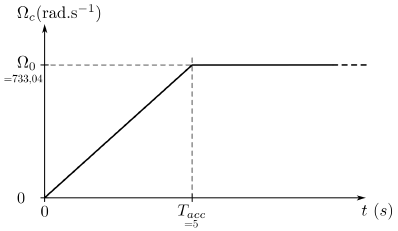
\includegraphics[width=\linewidth]{fig_50_01}
\caption{Représentation en coupe du banc BALAFRE \label{fig_50_01}}
\end{figure}
\fi


%\question{Conclure vis-à-vis de l’exigence concernant le risque de décrochage du
%moteur. Proposer deux solutions pour éviter le décrochage.}
%\ifprof
%\else
%\fi






\ifprof
\else
\begin{flushright}
\footnotesize{Corrigé  voir \ref{C1:02:50}.}
\end{flushright}%
\fi